\documentclass[border=6pt]{standalone}
\usepackage{tikz}
\usepackage[edges]{forest}
\usetikzlibrary{arrows.meta,positioning,calc,decorations.pathreplacing,shapes.geometric}
\begin{document}
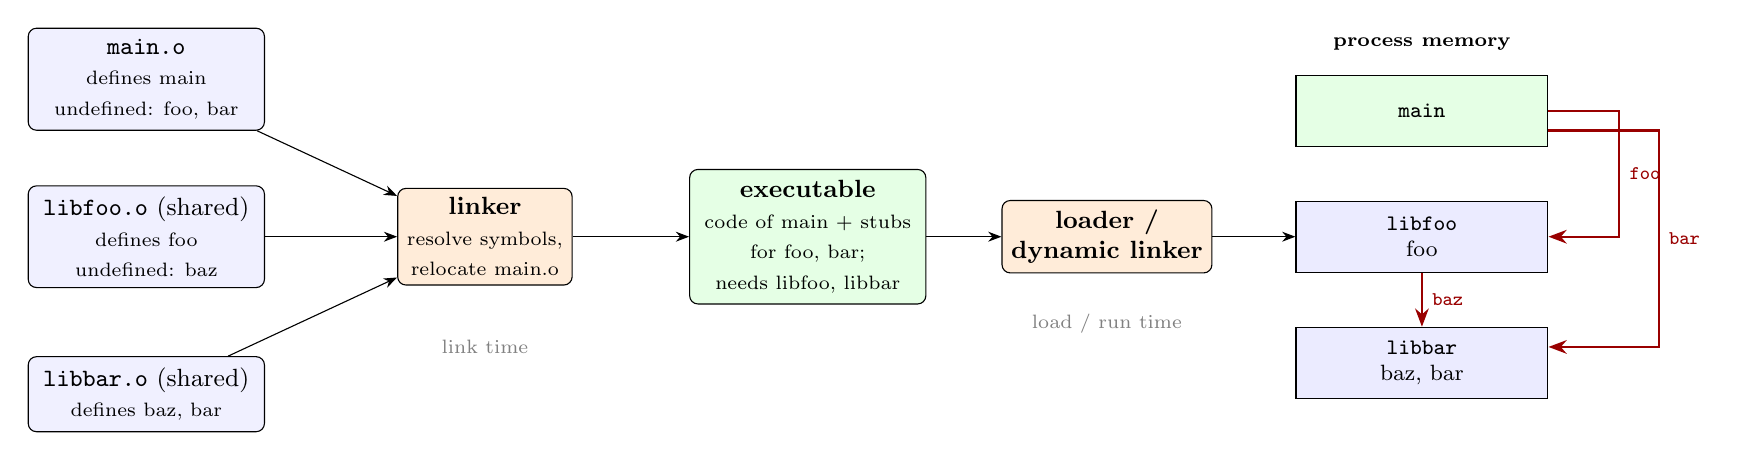
\begin{tikzpicture}[>=Stealth,font=\small,
 obj/.style={draw,rounded corners=3pt,fill=blue!6,align=center,minimum width=3.0cm,inner sep=4pt},
 pr/.style={draw,rounded corners=3pt,fill=orange!15,align=center,minimum width=2.2cm,minimum height=0.9cm},
 mem/.style={draw,minimum width=3.2cm,minimum height=0.9cm,align=center,font=\footnotesize}]
\node[obj] (m) at (0,2) {\texttt{main.o}\\{\scriptsize defines main}\\{\scriptsize undefined: foo, bar}};
\node[obj] (f) at (0,0) {\texttt{libfoo.o} (shared)\\{\scriptsize defines foo}\\{\scriptsize undefined: baz}};
\node[obj] (b) at (0,-2) {\texttt{libbar.o} (shared)\\{\scriptsize defines baz, bar}};
\node[pr] (ln) at (4.3,0) {\textbf{linker}\\{\scriptsize resolve symbols,}\\{\scriptsize relocate main.o}};
\node[obj,fill=green!10] (ex) at (8.4,0) {\textbf{executable}\\{\scriptsize code of main + stubs}\\{\scriptsize for foo, bar;}\\{\scriptsize needs libfoo, libbar}};
\node[pr] (ld) at (12.2,0) {\textbf{loader /}\\\textbf{dynamic linker}};
\draw[->] (m) -- (ln); \draw[->] (f) -- (ln); \draw[->] (b) -- (ln);
\draw[->] (ln) -- (ex); \draw[->] (ex) -- (ld);
\node[font=\scriptsize,gray] at (4.3,-1.4) {link time};
\node[font=\scriptsize,gray] at (12.2,-1.1) {load / run time};
% memory image
\node[mem,fill=green!10] (pm) at (16.2,1.6) {\texttt{main}};
\node[mem,fill=blue!8] (pf) at (16.2,0) {\texttt{libfoo}\\foo};
\node[mem,fill=blue!8] (pb) at (16.2,-1.6) {\texttt{libbar}\\baz, bar};
\node[font=\scriptsize\bfseries] at (16.2,2.45) {process memory};
\draw[->] (ld) -- (pf);
\draw[->,thick,red!60!black] (pm.east) -- ++(0.9,0) |- node[near start,right,font=\scriptsize]{\texttt{foo}} (pf.east);
\draw[->,thick,red!60!black] ([yshift=-0.25cm]pm.east) -- ++(1.4,0) |- node[near start,right,font=\scriptsize]{\texttt{bar}} ([yshift=0.2cm]pb.east);
\draw[->,thick,red!60!black] (pf.south) -- node[right,font=\scriptsize]{\texttt{baz}} (pb.north);
\end{tikzpicture}
\end{document}
